\documentclass{report}
\usepackage{graphicx}
\usepackage{hyperref}
\usepackage{placeins}
\usepackage{float}
\usepackage[acronym,nomain,nonumberlist]{glossaries}
\usepackage{titlesec}
\usepackage{enumerate}
\setcounter{tocdepth}{4}
\setcounter{secnumdepth}{4}
\makeatletter
\renewcommand{\thesection}{%
  \ifnum\c@chapter<1 \@arabic\c@section
  \else \thechapter.\@arabic\c@section
  \fi
  \let\Hy@linktoc\Hy@linktoc@none
}
\makeatother

\makeglossaries

\begin{document}

\tableofcontents
\newpage
\printglossaries
\newpage

%%%%%%%%%%%%%%%%%%%%%%%%%%%%%%%%%%%%%%%%%%%%%%%%%%%%%%%%%%%%%%%%%%%%%%%%%%%%%%%%%%%%%%%%%
% Acronym definitions
\newacronym{sdn}{SDN}{Software Defined Network}
\newacronym{mno}{MNO}{Mobile Network Operators}
\newacronym{ngmn}{NGMN}{Next Generation Mobile Networks}
\newacronym{sil}{SIL}{Service Instance Layer}
\newacronym{nsil}{NSIL}{Network Service Instance Layer}
\newacronym{e2e}{E2E}{End to End}
\newacronym{e2e}{E2E}{End to End}
\newacronym{fh}{FH}{Fronthaul}
\newacronym{bh}{BH}{Backthaul}
\newacronym{CN}{CN}{Core Network}
\newacronym{vi}{VI}{Virtual Infrastructure}
\newacronym{IaaS}{IaaS}{Infrastructure-as-a-Service}
\newacronym{NS}{NS}{Network Services}
\newacronym{VNF}{VNF}{Virtual Network Functions}
\newacronym{MANO}{MANO}{Management and Orchestration}
\newacronym{NBI}{NBI}{Northbound Interface}
\newacronym{SBI}{SBI}{Southbound Interface}
\newacronym{MTA}{MTA}{Multi-Tenancy Application}
\newacronym{NF}{NF}{Network Functions}
\newacronym{CP}{CP}{Control Plane}
\newacronym{UP}{UP}{User Plane}
\newacronym{AN}{AN}{Access Network}
\newacronym{RAT}{RAT}{Radio Access Technology}
\newacronym{NFV}{NFV}{Network Functions Virtualization}
\newacronym{eMBB}{eMBB}{enhanced Mobile Broadband}
\newacronym{mMTC}{mMTC}{massive Machine Type Communications}
\newacronym{URLLC}{URLLC}{Ultra‐Reliable Low‐Latency Communications}
\newacronym{VM}{VM}{Virtual Machines}
\newacronym{InP}{InP}{Infrastructure provider}
\newacronym{ONF}{ONF}{Open Networking Foundation}
\newacronym{SLA}{SLA}{Service Level Agreements}
\newacronym{KPI}{KPI}{Key Performance Indicators}
\newacronym{NFVI}{NFVI}{Network Functions Virtualization Infrastructure}
\newacronym{VIM}{VIM}{Virtual Infrastructure Manager}
\newacronym{VNFM}{VNFM}{Virtual Network Function Manager}
\newacronym{RO}{RO}{Resource Orchestrator}
\newacronym{NSO}{NSO}{Network Service Orchestrator}
\newacronym{NMS}{NMS}{Network Management System}
\newacronym{OSS/BSS}{OSS/BSS}{Operation/Business Support System}
\newacronym{EM}{EM}{Element Management}
\newacronym{IC}{IC}{Infrastructure SDN controller}
\newacronym{TC}{TC}{Tenant SDN controller}
\newacronym{EPC}{EPC}{Evolved Packet Core}
\newacronym{RAN}{RAN}{Radio Access Network}
\newacronym{QoS}{QoS}{Quality of Service}
\newacronym{QoE}{QoE}{Quality of Experience}
\newacronym{RRM}{RRM}{Radio Resource Management}
\newacronym{HSS}{HSS}{Home Subscriber System}
\newacronym{UDM}{UDM}{Unified Data Management}
\newacronym{AUSF}{AUSF}{Authentication Server Functions}
\newacronym{IoT}{IoT}{Internet of Things}
\newacronym{UPF}{UPF}{User Plane Processing Functions}
\newacronym{CPF}{CPF}{Control Plane Processing Functions}
\newacronym{AMF}{AMF}{Access and Mobility Management Function}
\newacronym{SMF}{SMF}{Session Management Function}
\newacronym{UDM}{UDM}{Unified Data Management}
\newacronym{NAS}{NAS}{Non‐Access Stratum}
\newacronym{RRC}{RRC}{Radio Resource Control}
\newacronym{RLC}{RLC}{Radio Link Control}
\newacronym{PDCP}{PDCP}{Packet Data Convergence Protocol}
\newacronym{API}{API}{Application Program Interface}


\section{Introduction}
Mobile networks are a key element of today's society, enabling communication, access
and information sharing. Moreover, traffic forecasts predict that the
demand for capacity will grow exponentially over the next years, mainly due to
video services. \\
However, as cellular networks move from being voice-centric to
data-centric, operators' revenues are not able to keep pace with the predicted
increase in traffic volume. Such pressure on operators' return on investment has
pushed research efforts toward designing for 5G novel mobile network solutions
able to open the door for new revenue sources. In this context, the network
slicing paradigm has emerged as a key 5G disruptive technology addressing this
challenge.\\
Network slicing for 5G allows \gls{mno} to open
their physical network infrastructure platform to the concurrent deployment
of multiple logical self-contained networks, orchestrated in different ways according
to their specific service requirements; such network slices are then
(temporarily) owned by tenants. The availability of this vertical market\footnote{A vertical market is a group of companies that serve each other's specialized needs and do not serve a broader market, therefore it is tightly focused on meeting the needs of one specific industry.} multiplies
the monetization opportunities of the network infrastructure as new
players may come into play (e.g., automotive industry, e-health) and an higher
infrastructure capacity utilization can be achieved by admitting network slice
requests and exploiting multiplexing gains.\\
With network slicing for 5G networks, different services (e.g., automotive,
mobile broadband, or tactile Internet) can be provided by different network slice
instances. Each of these instances consists of a set of virtual network functions
that run on the same infrastructure with a tailored orchestration. In this way,
very heterogeneous requirements can be provided on the same infrastructure, as
different network slice instances can be orchestrated and configured separately
according to their specific requirements. Additionally, this is performed in a
cost-efficient manner as the different network slice tenants share the same
physical infrastructure.\\
A network slice is defined by \gls{ngmn} as “\textit{a set of network functions, and
resources to run these network functions, forming a complete instantiated
logical network to meet certain network characteristics required by the Service
Instance(s)}”.\\
According to NGMN, the concept of network slicing involves three layers,
namely:
\begin{enumerate}[1]
\item \gls{sil};
\end{enumerate}
\begin{enumerate}[2]
\item \gls{nsil};
\end{enumerate}
\begin{enumerate}[3]
\item Resource Layer.
\end{enumerate}
The SIL represents the end user and/or
business services provided by the operator or the third-party service providers,
which are supported by the NISL. The NISL
is in turn supported by the resource layer, which may consist of the organic
resources such as compute, network, memory, storage, or it may be more
comprehensive as being a network infrastructure, or it may be more complex
as network functions.\\
Figure \ref{layers} depicts this concept where the resources at
the resource layer are sized to create several sub-network instances,
and network slice instances are formed that may use none, one, or multiple sub
network instances.\\
\begin{figure}
\centering
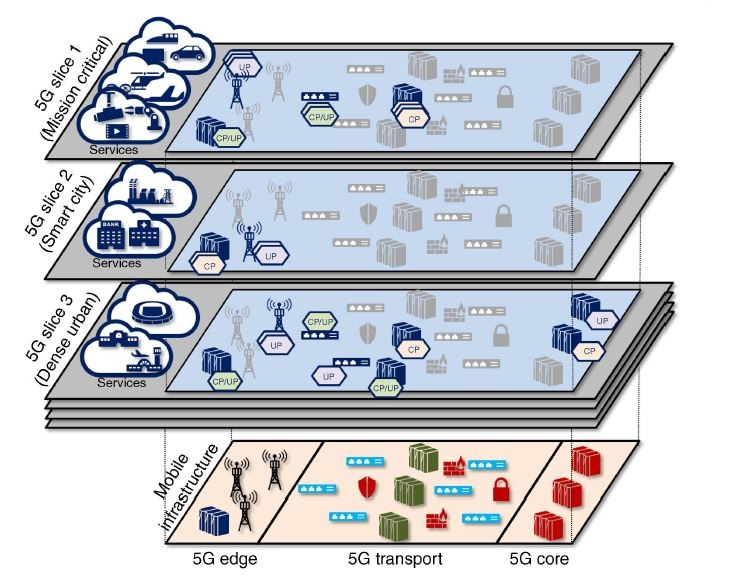
\includegraphics[scale=0.65]{pics/1.JPG}
\caption{Example of network slicing in 5G. \cite{al20185g}}
\label{layers}
\end{figure}The end goal of network slicing in 5G mobile networks is to be able to realize
\gls{e2e} network slices starting from the mobile edge, continuing
through the mobile transport (\gls{fh}/\gls{bh}), and up until
\gls{CN}. The allocation of a slice involves the selection of the
required functions, their constrained placement, the composition of the underlying infrastructure, and the allocation of the resources to fulfill the services' requirements, for example, bandwidth, latency, processing, resiliency.\\
The two main network slicing services that enable different degrees
of explicit control and are characterized by different levels of automation of the
mobile network slices management:
\begin{itemize}
\item The provision of \gls{vi} under the control and operation
of different tenants-in line with an \gls{IaaS} model\footnote{form of cloud computing that provides virtualized computing resources over the internet},
that is, creation of a network slice instance;
\end{itemize}
\begin{itemize}
\item The provision of tenant's owned \gls{NS}, that is, creation of a service instance.
In the former service, the deployment of a mobile network deals with the
allocation and deallocation of VIs.
\end{itemize}
The logical entities within a VI encompassing
a set of compute and storage resources are interconnected by a virtual, logical
network (i.e., virtual nodes are interconnected by virtual links over the substrate
network). The VIs can be operated by the tenant via different \gls{sdn} control
models. In the latter, NS are instantiated directly over a shared infrastructure,
and as a set of interrelated \gls{VNF} connected through
one or more VNF forwarding graphs.\\
Multi-tenancy is an characteristic that can be applied to both
kinds of services, guaranteeing separation, isolation, and independence between
different slices coupled with the efficient sharing of the underlying resources
for both VI and NS concepts.\\
In this context, a tenant is a logical entity owning and operating either one or more VIs or one or more network services. A tenant can be associated with an administrative entity (e.g., mobile virtual network operators) or
user of a given service (e.g., over-the-top service providers).\\
After this general overview of the situation, this essay will treat accurately all the necessary fundamental components in order to fully understand how 5G network slicing is actually built.


\newpage
\section{Architecture for Network Slicing} 
Starting from how an architecture for network slicing is conceptually made, it will be explained what it should achieve and involve, that is, the aspects of modularization, resource virtualization, virtual infrastructure, and network service management; they will be the main topics of this section.
\begin{figure}[h]
\centering
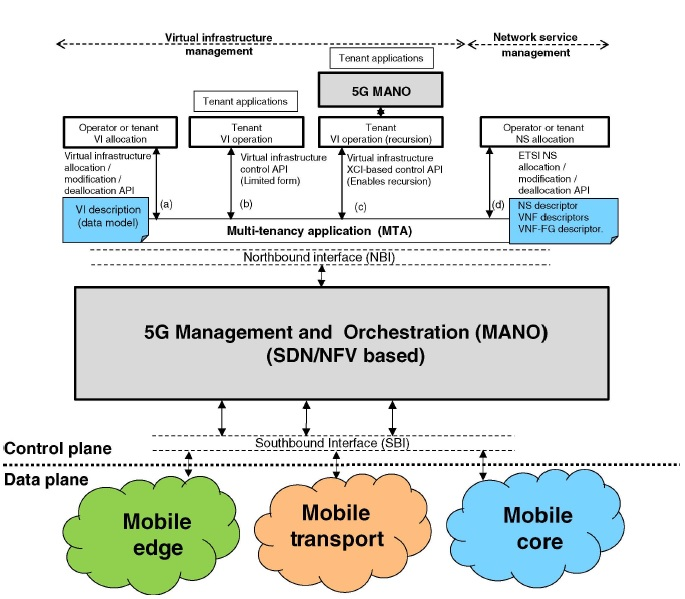
\includegraphics[scale=0.67]{pics/2.JPG}
\caption{Architecture for network slicing. \cite{al20185g}} 
\label{Arch}
\end{figure}
The design proposed in Fig. \ref{Arch} follows the SDN principles of:
\begin{itemize}
\item data and control plane fully decoupled;
\end{itemize}
\begin{itemize}
\item control logically centralized;
\end{itemize}
\begin{itemize}
\item applications having an abstracted view of resources and states.
\end{itemize}
The data plane is the resource layer which includes mobile edge, mobile transport, and core. The infrastructure is composed of links, forwarding nodes (e.g., switches and routers), cloud nodes (e.g., data centers), and so on, comprising a set of network, computing, and storage resources.\\
The control plane is divided into two layers: an application layer at the top and the 5G \gls{MANO} platform below. \\
The design of the MANO is based on the ETSI management and network orchestration framework with integrated SDN-based control. The MANO
provides an abstracted view of available resources and states and control, and
management functions to an ecosystem of applications, via a \gls{NBI}. On the other hand, the MANO is connected to the data plane
elements via a \gls{SBI} to execute control and management
functions (e.g., OpenFlow, SNMP, OVSDB) on the actual hardware components.
With respect to the \gls{MTA}, it implements the
multi-tenancy support by coordinating and managing tenants access to a shared
infrastructure, performing resource isolation between instances assigned to
different tenants, and delivering multi-tenancy-related services, such as the
allocation and operation of VIs, by means of dedicated \gls{API}s\footnote{An application program interface is code that allows two software programs to communicate with each other.} in cooperation
with the data plane, enforcing this logical separation. \\
As shown in Fig. \ref{Arch}
such APIs depend on the actual service: for the control of a VI or NS lifetime,
instantiation, modification, and deletion.

\subsection{Enablers and Design Principles}
Future 5G networks will be built on novel concepts that were not envisioned by the previous generation
network architectures. The revolution provided by the introduction of SDN
and \gls{NFV}\footnote{Although NFV and VNF are often used interchangeably, for the sake of clarity NFV is an overarching concept, while a VNF is building block of a NFV framework.} opens the door to a
large list of possible applications recalling that the latter focuses primarily on optimization of the network services, instead the former to separate the control and forwarding plane for a centralized view of the network. The fundamental parts involved in the network slicing realization for the future 5G networks are now discussed.

\subsubsection{Modularization}
The evolution of mobile communication systems towards 5G was intentionally aiming at achieving
architecture flexibility, heterogeneous accesses and vertical business integration, leveraging on NFV and SDN. To enable the design of logical architectures tailored to
performance and functional requirements of different use cases, the principle of architecture
modularization and network function decomposition was proposed at the earliest 5G research
stages.\\ 
\gls{NF}s are functional blocks
that provide specific network capabilities to support and realize the particular service(s). Generally implemented
as software instances running on infrastructure
resources, NFs can be physical (a combination
of specific hardware and software, defining a specific purpose-built physical appliance)
and/or virtualized (network function software is
decoupled from the hardware it runs on). \\
In particular, conventionally "monolithic" network functions are proposed to be split into basic modules, both for the \gls{CP} and \gls{UP}, thus allowing the definition of different logical architectures via the interconnection of
different subsets of CP and UP NFs.\\
In the process of decomposing the NFs into basic modules, the distinction between NFs relating to
the \gls{AN} and core network emerged. To minimize the dependency of the 5G
core on the access (and vice versa), and achieve the definition of a convergent network\footnote{Network convergence is the efficient coexistence of telephone, video and data communication within a single network.} providing
connectivity via a multitude of accesses not only including cellular radio, a different AN/CN functional split and an interface model are necessary.\\
Besides flexibility, the architecture modularization provides the essentials to support network
­slicing, as a network slice can be defined as an independent logical network shaped by the interconnection of a subset of NFs, composing both CP and UP, and which can be independently instantiated
and operated over physical or virtual infrastructure.

\subsubsection{Virtualization}
Virtualization is a key process for network slicing
as it enables effective resource sharing among
slices. Virtualization is the abstraction of resources
using appropriate techniques. The resource abstraction is the representation of a resource in terms of
attributes that match predefined selection criteria
while hiding or ignoring some of those irrelevant to such criteria, in order to simplify the
use and management of that resource in some
useful way. \\
The resources to be virtualized can
be physical or already virtualized, supporting a
recursive pattern with different abstraction layers.
Just as server virtualization makes \gls{VM}s independent of the underlying
physical hardware, network virtualization enables
the creation of multiple isolated virtual networks that
are completely decoupled from the underlying physical network and can safely run on top of it.
The framework consists of\ three kinds of actors:
\begin{itemize}
\item \gls{InP}: owns and manages a given physical network and its constituent resources. Such resources, in the form of
WANs and/or data centers, are virtualized and then offered through programming
interfaces to a single or multiple tenants.
\end{itemize}
\begin{itemize}
\item Tenant: leases virtual resources from one or
more InPs in the form of a virtual network,
where the tenant can realize, manage, and
provide network services to its users. A network service is a composition of NFs, and it
is defined in terms of the individual NFs and
the mechanism used to connect them.
\end{itemize}
\begin{itemize}
\item End user: consumes (part of) the services
supplied by the tenant, without providing
them to other business actors
\end{itemize}

\subsubsection{Orchestration}
Orchestration is also a key process for network
slicing. In its general sense, orchestration can be
defined as the concept of bringing together and coordinating different things into a coherent whole.
In a slicing environment, where the players involved
are so diverse, an orchestrator is needed to coordinate disparate network processes for
creating, managing, and delivering services.\\
According to the \gls{ONF},
orchestration is defined as "\textit{the continuing process of
selecting resources to fulfill client service demands
in an optimal manner}". The idea of optimal refers
to the optimization policy that governs orchestrator behavior, which is expected to meet all the service level agreements \gls{SLA}s associated with clients (e.g., tenants or end users)
that request services. The term continuing means
that available resources, service demands, and optimization criteria may change in time. \\
Interestingly, orchestration is also referred to as the defining
characteristic of an SDN controller. Note that client
is a term used in the SDN context.
The ONF states that the orchestrator functions
include client-specific service demand validation,
resource configuration, and event notification.
However, in network slicing, orchestration cannot be performed by a single centralized entity,
not only because of the complexity and the
scope of orchestration tasks, but also because it
is necessary to maintain management independence and support the possibility of recursion. \\
A framework in which each virtualization
actor has an entity performing orchestration functions seems more suitable to satisfy the
above requirements. The entities should exchange
information and delegate functionalities between
them to ensure that the services delivered at a
certain abstraction layer satisfy the required performance levels with optimal resource utilization.

\paragraph{Isolation}\mbox{}\\
Strong isolation is a major requirement that must
be satisfied to operate parallel slices on a common shared underlying substrate. The isolation
must be understood in terms of:
\begin{itemize}
\item Performance: Each slice is defined to meet particular service requirements, usually expressed in the
form of \gls{KPI}s. Performance isolation is an E2E issue and has to ensure
that service-specific performance requirements are
always met on each slice, regardless of the congestion and performance levels of other slices.
\end{itemize}
\begin{itemize}
\item Security and privacy: Attacks or faults occurring in one slice must not have an impact on
other slices. Moreover, each slice must have
independent security functions that prevent unauthorized entities to have read or write access to
slice-specific configuration/management/accounting information, and be able to record any of
these attempts, whether authorized or not.
\end{itemize}
\begin{itemize}
\item Management: Each slice must be independently managed as a separate network.
\end{itemize}
To achieve isolation, a set of appropriate, consistent policies and mechanisms have to be defined
at each virtualization level, following the recursion
principle introduced earlier. The policies contain lists of rules that describe how different manageable entities must be properly isolated, without delving into how this can be achieved.
To fully realize the
required isolation level and so this shows that the interplay of both virtualization and orchestration is actually needed.




\subsubsection{SDN: Software-Defined Network}
In a software-defined network, a network engineer or administrator can shape traffic from a centralized control console without having to touch individual switches in the network. The centralized SDN controller directs the switches to deliver network services wherever they are needed, regardless of the specific connections between a server and devices. This process is a move away from traditional network architecture, in which individual network devices make traffic decisions based on their configured routing tables.\\
The SDN architecture comprises an intermediate control plane that dynamically configures and abstracts the underlying
forwarding plane resources so as to deliver tailored services to clients located in the application plane. This is
well aligned with the requirements of 5G network
slicing, which needs to satisfy a wide range of service demands. Then, the SDN architecture is an appropriate
tool for supporting the key principles of slicing.\\
The major SDN components are resources and controllers. For
SDN, a resource is anything that can be utilized to
provide services in response to client requests. This
includes infrastructure resources\footnote{Heterogeneous hardware and necessary software for hosting and connecting NFs. They include computing hardware,
storage capacity, networking resources (e.g., links
and switching/routing devices enabling network
connectivity), and physical assets for radio access.
} and NFs, but also
network services, in application of the recursion
principle described earlier. A controller is a logically centralized entity instantiated in the control
plane which operates SDN resources at runtime
to deliver services in an optimal way. Therefore,
it mediates between clients and resources, acting simultaneously as server and client via client
and server contexts, respectively. Both contexts
are conceptual components of an SDN controller
enabling the server-client relationships:
\begin{itemize}
\item Client context: Represents all the information the
controller needs to support and communicate with
a given client. It comprises a Resource Group and
a Client support function. The Resource Group contains an abstract, customized view of all the resources that the controller, through one of its northbound
interfaces, offers to the client, in order to deliver
on its service demands and facilitate its interaction
with the controller. Client support contains all that
is necessary to support client operations, including
policies on what the client is allowed to see and do and service-related information to map actions
between the client and the controller.
\end{itemize}
\begin{itemize}
\item Server context: Represents all the information the controller needs to interact with a set of
underlying resources, assembled in a Resource
Group, through one of its southbound interfaces.
\end{itemize}
The process of transforming the set of
Resource Groups accessed through server contexts to those defined in separate client contexts
is not straightforward, and it requires the SDN
controller to perform virtualization and orchestration functions.\\
When performing the virtualization function, the
SDN controller carries out the abstraction and the
aggregation/partitioning of the underlying resources. Thanks to virtualization, each client context provides a specific Resource Group that can be used by the client associated with that context to realize
its service(s). Through orchestration, the SDN controller optimally dispatches the selected resources
to such separate Resource Groups. \\
The interplay of both controller functions enables the fulfillment
of the diverging service demands from all clients
while preserving the isolation among them.\\
The SDN architecture also includes an administrator. Its tasks consist of instantiating and configuring the entire controller, including the creation
of both server and client contexts and the installation of their associated policies.\\
The SDN architecture naturally supports slicing, as the client context provides the complete abstract set of resources
(as a Resource Group) and the supporting control
logic that constitute a slice, including the complete
collection of related client service attributes.\\
Another key functional aspect that makes SDN
architecture ideal to embrace 5G slicing is recursion. Because of the different abstraction layers
that the recursion principle enables, the SDN
control plane can involve multiple hierarchically
arranged controllers that extend the client-server
relationships at several levels. According to
these premises, it is evident that SDN can support a
recursive composition of slices. This implies that
the resources (i.e., Resource Group) a given controller delivers to one of its clients in the form of a
dedicated slice (i.e., client context) can, in turn, be
virtualized and orchestrated by such a client in the
case of being an SDN controller. In this way, the new
controller can utilize the resource(s) it accesses via
its server context(s) to define, scale, and deliver
new resources (and hence new slices) to its own
clients, which might also be SDN controllers.


\subsubsection{NFV: Network Functions Virtualization}
Although the SDN architecture described above
gives a comprehensive view of the control plane
functionalities enabling slicing, it lacks capabilities
to efficiently manage the life cycle of
network slices and its resources. \\
VNFs, generally speaking, are virtualized tasks formerly carried out by proprietary, dedicated hardware. VNFs move individual network functions out of dedicated hardware devices into software that runs on commodity hardware. These tasks, used by both network service providers and businesses, include firewalls, domain name system, caching or network address translation and can run as virtual machines. In this respect, the NFV architecture is ideal to play
this role, as it manages the infrastructure resources
and orchestrates the allocation of such resources
needed to realize VNFs and network services.\\
To benefit from the management and orchestration functionalities of NFV, appropriate cooperation between SDN and NFV is required.
However, embracing SDN and NFV architectures
into a common reference framework is not an
easy task. ETSI presents a framework
to integrate SDN within the reference NFV architecture. This framework incorporates two SDN
controllers, one logically placed at the tenant and
another at the InP level. The NFV architecture comprises the following
entities:\\
\begin{itemize}
\item \gls{NFVI}: A collection of resources used to
host and connect the VNFs. While the broad scope of SDN makes resource a generic concept,
the current resource definition in the NFV framework comprises only the infrastructure resources.
\end{itemize}
\begin{itemize}
\item VNFs: Software-based implementations of NFs that run over the NFVI.
\end{itemize}
\begin{itemize}
\item \gls{MANO}: Performs all the virtualization-specific management, coordination, and automation tasks in the NFV architecture. The MANO framework comprises three functional blocks:
\begin{itemize}
\item \gls{VIM}: responsible for controlling and managing the NFVI resources.
\end{itemize}
\begin{itemize}
\item \gls{VNFM}: performs configuration and life cycle management of the VNF(s) on its domain.
\end{itemize}
\begin{itemize}
\item Orchestrator: According to ETSI, it has two set of functions performed by the Resource \gls{RO} and \gls{NSO}, respectively. The RO orchestrates the NFVI resources across (potentially different) VIMs. The NSO performs the life cycle management of network
services using the capabilities provided by the
RO and the (potentially different) VNFMs.
\end{itemize}
\end{itemize}
\begin{itemize}
\item \gls{NMS}: Framework performing the general network management tasks. Although its functions are orthogonal to those defined in MANO, NMS is expected to interact with MANO entities by means of a clear separation of roles. NMS comprises:
\begin{itemize}
\item \gls{EM}: responsible for the fault, configuration,
accounting, performance, and security of a VNF.
\end{itemize}
\begin{itemize}
\item \gls{OSS/BSS}: a collection of systems and manage-
ment applications that network service providers use to provision and operate their network
services. In terms of the roles we considered
earlier, tenants would run these applications.
\end{itemize}
\end{itemize}
The ETSI proposal includes two SDN controllers
in the architecture. Each controller centralizes
the control plane functionalities and provides an
abstract view of all the connectivity-related components it manages. These controllers are:
\begin{itemize}
\item \gls{IC}: Sets up
and manages the underlying networking resources to provide the required connectivity for communicating the VNFs.
Managed by the VIM, this controller may change
infrastructure behavior on demand according to
VIM specifications adapted from tenant requests.
\end{itemize}
\begin{itemize}
\item \gls{TC}: instantiated in
the tenant domain as one of the VNFs or as
part of the NMS, this second controller dynamically manages the pertinent VNFs used to realize
the tenant’s network service(s). These VNFs are
the underlying forwarding plane resources of the
TC. The operation and management tasks that the
TC carries out are triggered by the applications
running on top of it (e.g. the OSS).
\end{itemize}
Both controllers manage and control their
underlying resources via programmable southbound interfaces, implementing protocols like
OpenFlow, NETCONF, and I2RS. However, each
controller provides a different level of abstraction. While the IC provides an underlay to support
the deployment and connectivity of VNFs, the
TC provides an overlay comprising tenant VNFs
that, properly composed, define the network service(s) such a tenant independently manages on
its slice(s). These different resource views each
controller offers through its interfaces have consequences on the way they operate. On one side,
the IC is not aware of the number of slices that utilize the VNFs it connects, nor the tenant(s) which
operate(s) such slices. On the other side, for the
TC the network is abstracted in terms of VNFs,
without notions of how those VNFs are physically
deployed. \\
Despite their different abstraction levels,
both controllers have to coordinate and synchronize their actions. Note that the service and
tenant concept mentioned here can be extended
to higher abstraction layers by simply applying the
recursion principle.\\
Finally an overall description of the system is given by Fig. \ref{integral}.
\begin{figure}[h]
\centering
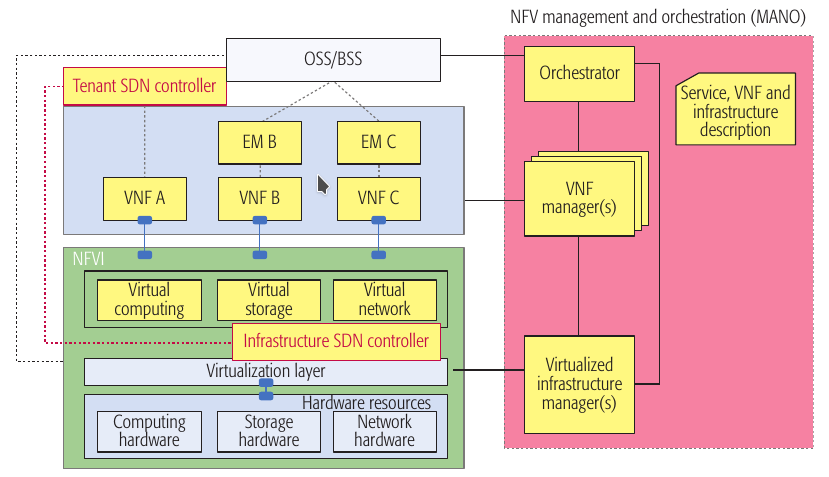
\includegraphics[scale=0.56]{pics/integral.png} 
\caption{Integrating SDN controllers into the reference NFV architectural framework. \cite{ordonez2017network}}
\label{integral}
\end{figure}



\newpage
\section{Network Slicing} 
Now we have all the players to look inside what NGMN has proposed as the concept of network slicing with the target to create tenant or service‐specific networks. While legacy systems host multiple telecommunication
services, such as mobile broadband, voice, SMS, on the same mobile network architecture, for
instance composed of Long Term Evolution radio access and the \gls{EPC},
future 5G networks should also support shared or dedicated logical architectures customized to the
respective telco or vertical services, such as \gls{eMBB}, vehicular communications, \gls{URLLC}, and \gls{mMTC}. These services need very different KPIs that are
hard to be fulfilled by legacy systems, as they are characterized by monolithic network elements that
have tightly coupled hardware, software, and functionality. \\
Future architectures, as already explained, leverages the decoupling of software‐based network functions from the underlying infrastructure resources by
means of utilizing different resource abstraction technologies.
Furthermore, exploiting modularization, well‐known resource sharing technologies such as multiplexing and multitasking ( e.g.
wavelength division multiplexing or radio scheduling), can be advantageously complemented
by softwarization techniques. Multitasking and multiplexing allow sharing
physical infrastructure that is not virtualized. NFV and SDN allow different tenants to share the
same general‐purpose hardware. 
\begin{figure}[H]
\centering
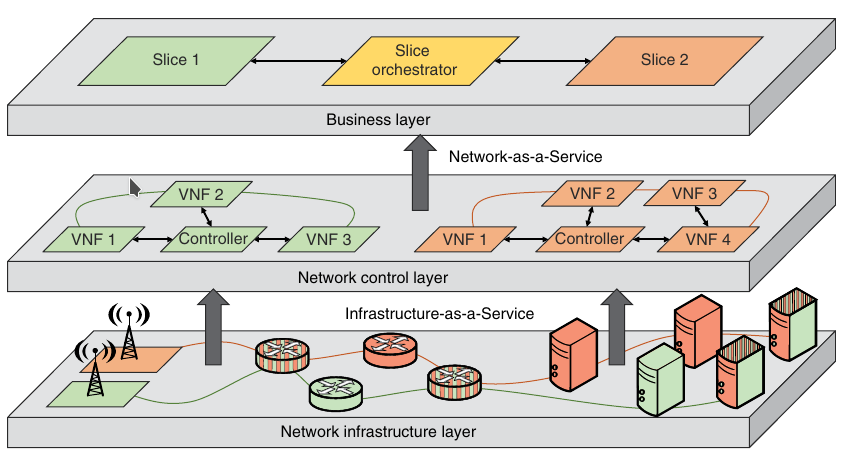
\includegraphics[scale=0.55]{pics/slice.png}
\caption{An example of a network‐sliced architecture. \cite{al20185g}} 
\label{slice}
\end{figure}
In combination, these technologies allow building fully decoupled E2E networks on top of a common, shared infrastructure. Consequently, multiplexing will not happen on the network level anymore, but on the
infrastructure level, as depicted in Fig. \ref{slice}, yielding better \gls{QoS} or \gls{QoE} for the subscriber (as different slices will have tailored orchestration for a given
service) as well as improved levels of network operability for the mobile service provider or mobile
network operator.\\
In principle, a network slice is a logical network that provides specific network capabilities and
network characteristics and comprises NFs, computing and networking resources to meet the
­performance requirements of the tenants, for instance verticals. This comprises both \gls{RAN} and CN NFs and, depending on the degree of freedom that a tenant may have, also
the MANO components. A network slice may be dedicated to a
specific tenant or partially shared by several tenants that have the same performance requirements
but different security or policy settings. \\
The decoupling between the virtualized and the physical
infrastructure allows for the efficient scaling of the slices, hence suggesting the
economic viability of this approach that can adapt the used resources on demand.\\
The 5G atom proposed in Fig. \ref{atom} summarizes the discussion: use cases are in the center; the layers, from the center out, represent the requirements of the 5G use cases, the concepts that will allow network
operators to satisfy the requirements, the technologies that enable the implementation of
the concepts, and the novelties, that is, technologies that can be easily implemented due
to softwarization and virtualization techniques.
\begin{figure}[h]
\centering
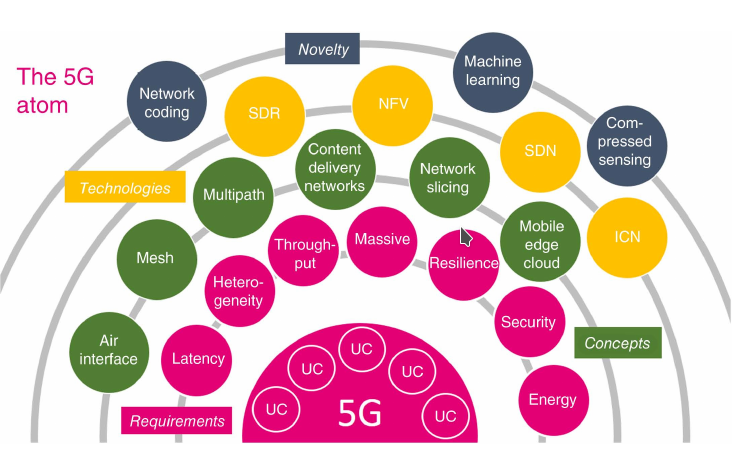
\includegraphics[scale=0.63]{pics/5g_atom.png} 
\caption{5G atom representation. \cite{marsch20185g}}
\label{atom}
\end{figure}


\subsection{Main Services Types}
The main 5G service types typically considered are:
\begin{itemize}
\item Enhanced mobile broadband (eMBB): related to human‐centric and enhanced access to multimedia content, services and data with improved performance and increasingly seamless user experience. This service type, which can be seen as an evolution of the services nowadays provided by
4G networks, covers UCs with very different requirements, e.g. ranging from hotspot UCs characterized by a high user density, very high traffic capacity and low user mobility, to wide area coverage cases with medium to high user mobility, but the need for seamless radio coverage practically
anywhere and anytime with visibly improved user data rates compared to today;
\end{itemize}
\begin{itemize}
\item Ultra‐reliable and low-latency communications (URLLC): related to UCs with stringent requirements for capabilities such as latency, reliability and availability. Examples include the wireless
control of industrial manufacturing or production processes, remote medical surgery, distribution automation in a smart grid, transportation safety, etc. It is expected that URLLC services will provide a main part of the fundament for the 4th industrial revolution (often referred to as
Industry 4.0) and have a substantial impact on industries far beyond the information and communication technology industry;
\end{itemize}
\begin{itemize}
\item Massive machine‐type communications (mMTC): capturing services that are characterized by
a very large number of connected devices typically transmitting a relatively low volume of non delay‐sensitive data. However, the key challenge is here that devices are usually required to be
low-cost, and have a very long battery lifetime. Key examples for this service type would be logistics applications (e.g., involving the tracking of tagged objects), smart metering, or for instance
agricultural applications where small, low‐cost and low‐power sensors are sprinkled over large
areas to measure ground humidity, fertility, etc.
\end{itemize}
The concept of network slicing will be implemented at the beginning of the 5G era in order to realize these main services as slices and their 8 most important KPI are the following:
\begin{itemize}
\item Peak data rate, referring to the maximum achievable data rate under ideal conditions per user or
device in bits per second. The minimum 5G requirements for peak data rate are 20 Gbps in the
downlink and 10 Gbps in the uplink;
\end{itemize}
\begin{itemize}
\item User experienced data rate, referring to the achievable data rate that is available ubiquitously
across the coverage area to a mobile user or device in bits per second. This KPI corresponds to the
5\% point of the cumulative distribution function of the user throughput, and represents
a kind of minimum user experience in the coverage area. This requirement is set by ITU‐R to
100 Mbps in the DL and 50 Mbps in the UL;
\end{itemize}
\begin{itemize}
\item Average spectral efficiency, also known as spectrum efficiency and defined as the average data
throughput per unit of spectrum resource and per cell in bps/Hz/cell. Again, the minimum require-
ments depend on the test environments as follows:
\begin{itemize}
\item Indoor Hotspot: 9 bps/Hz/cell in the DL, 6.75 bps/Hz/cell in the UL;
\end{itemize}
\begin{itemize}
\item Dense Urban: 7.8 bps/Hz/cell in the DL, 5.4 bps/Hz/cell in the UL;
\end{itemize}
\begin{itemize}
\item Rural: 3.3 bps/Hz/cell in the DL, 1.6 bps/Hz/cell in the UL.
\end{itemize}
\end{itemize}
\begin{itemize}
\item Area traffic capacity, defined as the total traffic throughput served per geographic area in Mbps/m2.
ITU‐R has defined this objective only for the indoor hotspot case, with a target of 10 Mbps/m2 for
the downlink;
\end{itemize}
\begin{itemize}
\item User plane latency, given as the contribution of the radio network to the time from when the
source sends a packet to when the destination receives it. The one‐way end‐to‐end latency
requirement is set to 4 ms for eMBB services and 1 ms for URLLC;
\end{itemize}
\begin{itemize}
\item Connection density, corresponding to the total number of connected and/or accessible devices
per unit area. ITU‐R has specified a target of 1 000 000 devices per km$^2$ for mMTC services;
\end{itemize}
\begin{itemize}
\item Energy efficiency, on the network side referring to the quantity of information bits transmitted to or received from users, per unit of energy consumption of the RAN, and on the device side to the
quantity of information bits per unit of energy consumption of the communication module,both cases in bits/Joule. The specification given by ITU‐R in this respect is that IMT‐2020 air interfaces must have the capability to support a high sleep ratio and long sleep duration;
\end{itemize}
\begin{itemize}
\item Mobility, here defined as the maximum speed at which a defined QoS and
seamless transfer between radio nodes which may belong to different layers and/or radio access
technologies can be achieved. For the rural test environment, the normalized traffic channel link
data rate at 500 km/h, reflecting the average user spectral efficiency, must be larger than 0.45 bps/Hz
in the uplink.
\end{itemize}
The following web-spider diagrams in Fig. \ref{cap1}, \ref{cap2}, sum up optimally these capabilities and how they have to be split to realize each particular slice
\begin{figure}[h]
\centering
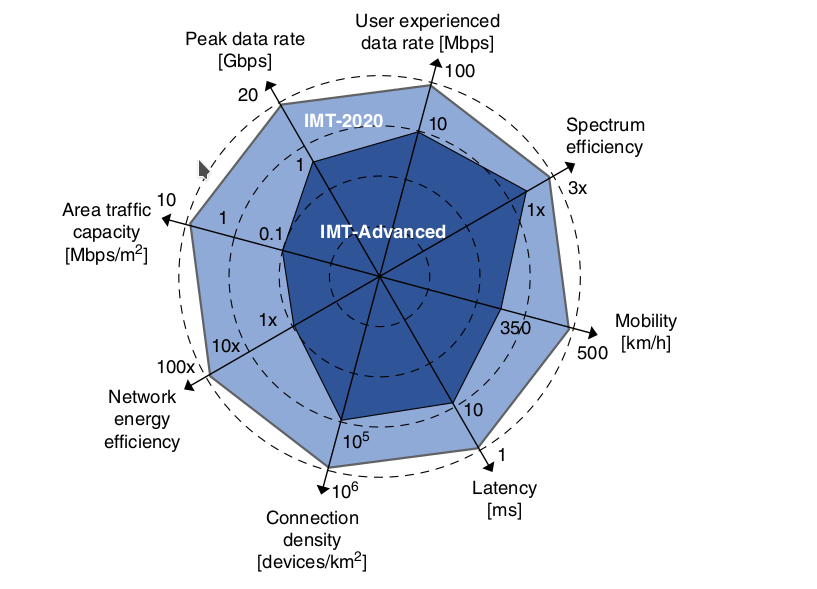
\includegraphics[scale=0.4]{pics/capabilities1.png}
\caption{Capabilities to be achieved. \cite{al20185g}} 
\label{cap1}
\end{figure}
\begin{figure}[H]
\centering
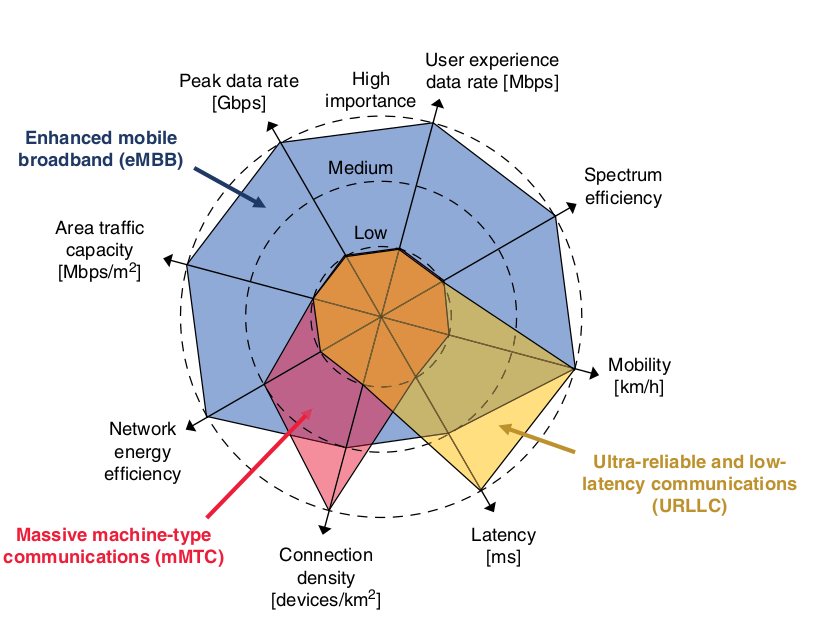
\includegraphics[scale=0.4]{pics/capabilities2.png}
\caption{How capabilities are divided for each slice. \cite{al20185g}} 
\label{cap2}
\end{figure}


\subsection{Example}
An illustrative example for deploying multiple network slice instances in a
mixed environment consisting of public, i.e. mobile network operator owned, networks and
private network infrastructure owned by a vertical enterprise. The infrastructure is used to commission an mMTC network slice and two eMBB network slices. 

\subsubsection{5G Services on Factory Premises}
A process automation use case from industrial manufacturing is considered. Traffic is composed of sensor readings, actuator control signaling, and eMBB services providing access to local as well as remote applications (e.g. augmented reality for machine maintenance).\\
In a process automation environment, \gls{IoT} devices include actuators, such as pumps, valves and
sensors for capturing heterogeneous physical and logical quantities. The latter may for instance include sensors for supporting maintenance processes or for critical safety
applications, aiming to improve the overall operational efficiency and safety of the factory. When
connecting such IoT devices, latency and bandwidth requirements can be very diverse. Such a setup
requires two types of network slices, one covering machine‐type communications for IoT devices
and one covering eMBB traffic from smartphones, tablets and similar terminals. 
\begin{figure}
\centering
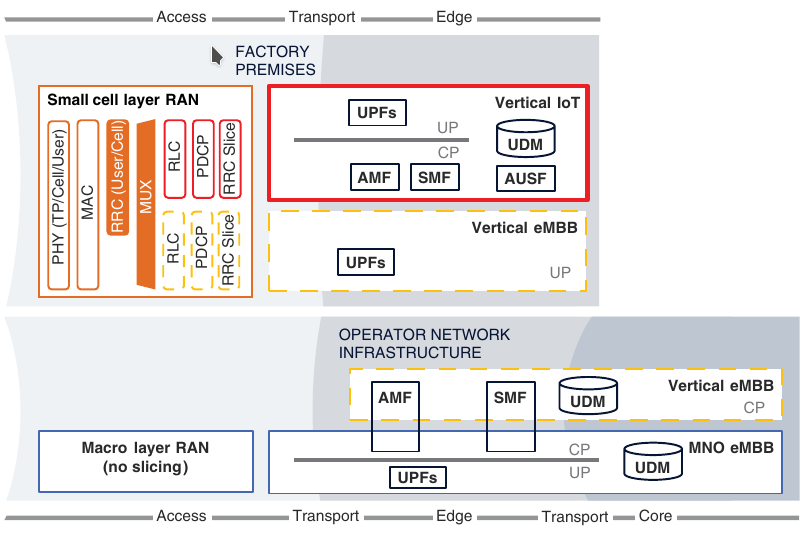
\includegraphics[scale=0.56]{pics/example.png}
\caption{E2E network slice example for 5G services on factory premises. \cite{al20185g}}
\label{exem} 
\end{figure}
Figure \ref{exem} shows an example scenario with two E2E network slices (mMTC and vertical eMBB) for the factory owner (also
referred to as “vertical”) as well as an eMBB network slice for the MNO. The network slices run MNO infrastructure as well as the vertical’s telecommunication infrastructure on the factory premises.

\subsubsection{Ownership of Infrastructure, Spectrum, and Subscriber Data}
In the given scenario, the vertical provides the small cell layer RAN equipment for all network slices
that require coverage on the factory premises, i.e., both the IoT slice and vertical eMBB slice. Beyond
the RAN, this includes the transport network and edge cloud resources, such as general purpose
hardware for computing and storage. For operating the small cell layer RAN, the vertical rents dedicated spectrum resources from the MNO, such as higher frequency spectrum (e.g., above 6 GHz)
with coverage strictly limited to the factory premises. For the vertical eMBB service, both small cell
layer RAN and, if required, the MNO‐provided macro layer RAN are utilized. \gls{RRM} functions for the
macro layer strictly remain under control of the MNO, which further owns a 5G‐compatible network infrastructure consisting of centralized datacenters and distributed edge clouds comprising general-purpose as well as application‐specific hardware.\\ Subscriber information data including long‐term security credentials are in possession of the vertical for the IoT devices. This assures full isolation of
the vertical’s IoT subscriber information from the MNO. For the eMBB subscribers, the MNO holds
the corresponding data for own eMBB subscribers as well as vertical eMBB subscribers.

\subsubsection{Domain‐specific Network Slice Deployment}
Regarding the deployment of the individual network slices, the mMTC network slice deploys all functions in the domain of the vertical, and it is only used by IoT
devices that are registered in the vertical’s \gls{HSS} or \gls{UDM} and \gls{AUSF}. These devices are mostly stationary and never
leave the factory premises. The small cell layer RAN as well as the IoT‐specific \gls{UPF}s and \gls{CPF}s, in particular \gls{AMF} and \gls{SMF}, are operated locally under full control of
the vertical. Since also the security mechanisms are strictly realized locally, the entire network slice operates in the shielded factory environment without exposure of any data to the MNO. In contrast, the vertical eMBB slice is deployed
in an inter‐domain manner: the CN control plane is shared with the MNO
eMBB network slice and operated by the MNO outside the factory, including AMF and SMF as well
as AUSF and \gls{UDM} for authentication towards the core network and \gls{NAS}
ciphering and integrity protection, respectively. \\
Regarding the transport network, independent slices
with guaranteed levels of isolation and security are used by both the vertical and the MNO. In the vertical’s small cell layer RAN, on the factory premises, physical and MAC layer in the UP
and \gls{RRC} in the CP are shared by both slices. This approach limits the complexity because resource
multiplexing is implemented across all network slices on MAC level, forcing each network slice to
make use of the same efficient flexible RAN implementation. On the other hand, each network slice
may still customize the operation through configuration and parameterization of \gls{RLC}, \gls{PDCP}, and RRC‐Slice functions, RRM for the small cell layer realizes resource allocation
according to the defined SLAs for the mMTC and eMBB slices of the vertical.


\subsection{Actual Implementations}
Some early trials have been conducted demonstrating network slicing with
cross-industry collaboration among operators, vendors, and vertical industries.
Two specific examples are given here.
\begin{itemize}
\item Deutsche Telekom and Huawei demonstration of E2E autonomous network slicing. In this demo, eMBB, mMTC and uRLLC are envisaged as network classes that could be built as slices.
E2E network slicing included not only the core network and RAN, but also
interconnecting transport networks. The demo implements E2E network slicing automation based on service oriented network auto creation. It uses software-defined topology, software-defined protocol, and
software-defined resource allocation to ensure the automatic implementation of slice management, service deployment, resource scheduling, and fault recovery.
\end{itemize}
\begin{itemize}
\item SK Telecom, Deutsche Telekom and Ericsson have jointly built
and demonstrated a trial network on federated network slicing for roaming, making SK Telecom and DT network slices available in each operators footprint, connecting South Korea and Germany. The demonstration
was hosted at Deutsche Telekom's corporate R\&D center in Bonn, Germany and Sk Telecoms 5G testbed at Yeongjongdo (the BMW driving center) in Korea. The
demo featured an industrial maintenance use case involving a repair worker
communicating via augmented reality with support colleagues in a visited network. The scenario used local breakout and edge cloud to enable
the best service experience in terms of latency and throughput for the augmented reality
repairman.
\end{itemize}


\phantomsection 
\addcontentsline{toc}{chapter}{Bibliography} 

\newpage
\nocite*
\bibliographystyle{plain}
\bibliography{biblist}

\end{document}